\documentclass[conference]{IEEEtran}
% Supplementary material for the ICME submission (weave.tex). Not page-limited;
% upload as a single zip together with nothing identifying.
\usepackage{cite}
\usepackage{amsmath,amssymb}
\usepackage{graphicx}
\usepackage{booktabs}
\usepackage{xcolor}
\usepackage[hyphens]{url}
\graphicspath{{figures/}}
\newcommand{\dinos}{DINO-S}
\newcommand{\dinoc}{DINO-C}
\newcommand{\clips}{CLIP-S}
\renewcommand{\thesection}{S\arabic{section}}
\renewcommand{\thetable}{S\arabic{table}}
\renewcommand{\thefigure}{S\arabic{figure}}

\begin{document}
\title{Supplementary Material for\\``WEAVE: Escaping the Identity Shortcut in\\Lightweight Style Transfer with Wavelets''}
\author{Anonymous ICME submission}
\maketitle

\begin{abstract}
This supplement documents the evaluation protocol, the resolved training configuration, the
internal stopping probe, per-epoch curves for every seed and retrained ablation, sensitivity
sweeps, reference-pool and ArtFID audits, structure-preservation measurements, the
high-frequency route probes that motivated the final architecture, and the frozen SD1.5 plug-in.
Section, table, and figure numbers prefixed with ``S'' refer to this document; all others refer
to the main paper.
\end{abstract}

\section{Evaluation Protocol}
\label{sec:protocol}

\noindent\textbf{D5-512.} Distinct5-WikiArt at 512\,px contains Early Renaissance, Impressionism,
Minimalism, Rococo, and Ukiyo-e, with 3{,}600 training and 150 test images per style. Each of 30
test sources per style is sent to all five targets, giving 750 ordered requests; the 150
same-style requests are kept as calibration rows. Training uses a frozen prototype pairing cache
built from training latents only.

\noindent\textbf{P2A-256.} A 256\,px five-domain grid over photo, Monet, Van Gogh, C\'ezanne, and
Hayao, evaluated with the same ordered logic. Several external baselines only provide the 600
off-diagonal requests on this board; their scores are averaged over the images they provide, and
image counts are recorded with every score.

\noindent\textbf{R5-WikiArt.} Five randomly drawn WikiArt families (Cubism, Expressionism, Pop
Art, Romanticism, Symbolism) at 512\,px with the same 750-request layout.

\noindent\textbf{Metrics.} \dinos{} is the mean over requests of the maximum cosine similarity
between the DINOv2-small CLS feature of the output and the CLS features of up to 30 held-out
references of the target style (the source is excluded from the pool). \clips{} is the CLIP
ViT-B/32 cosine similarity to the target-style prototype. \dinoc{} is the DINOv2-small CLS cosine
between output and source. LPIPS uses the AlexNet backbone. Images are resized to 224 and
center-cropped for DINO; metric post-processing is disabled.

\noindent\textbf{IDT and TGT.} For source $x$ and target style $s$, $y_{\mathrm{IDT}}=x$ and
$y_{\mathrm{TGT}}=r_s$, where $r_s$ is the first image in the deterministic held-out reference
order of style $s$, reused for every source sent to $s$. TGT depends on the requested style but
not on the source, and is never an input to any method. We read the bracket
\begin{equation}
\begin{aligned}
M_{\mathrm{style}}(y)&>M_{\mathrm{style}}(y_{\mathrm{IDT}}),\\
\mathrm{LPIPS}(y,x)&<\mathrm{LPIPS}(y_{\mathrm{TGT}},x),\\
\dinoc(y,x)&>\dinoc(y_{\mathrm{TGT}},x)
\end{aligned}
\end{equation}
inequality by inequality and never combine it into a weighted score. IDT and TGT are empirical
anchors, not bounds: crossing one prompts visual inspection rather than a verdict. TGT reaches
\dinos{} 1.000 by construction because $r_s$ belongs to the reference pool. Using each of the
first five deterministic exemplars as $r_s$ moves TGT LPIPS within 0.752--0.783 and TGT \dinoc{}
within 0.189--0.246 on D5; StyleAligned (LPIPS 0.869) lies beyond every one of these anchors.

\section{Implementation}
\label{sec:impl}

Table~\ref{tab:config} lists the resolved configuration of the reported D5 model. The frozen SD1.5
EMA VAE (84M parameters, latent scale 0.18215) is used only to encode training latents once and
to decode outputs. The velocity network has four main residual blocks (plus two high-resolution
and two decoder blocks) at width 64 and time embedding 256; with the orientation-specific
target-HF route it has 1{,}037{,}087 trainable parameters (873{,}680 without the route).

\begin{table}[t]
\centering
\caption{Resolved configuration of the reported D5-512 run.}
\label{tab:config}
\footnotesize
\begin{tabular}{@{}ll@{}}
\toprule
Field & Value \\
\midrule
Decomposition & one-level Haar on the VAE latent \\
Endpoint & source-aligned LL, $\alpha=0.3$; target LH/HL/HH \\
Band weights & LL 0.3, LH 1.0, HL 1.0, HH no head \\
Path & $t\sim\mathcal U[0,1]$, $\sigma=0.02$ perturbation \\
Target-HF route & pooled LH/HL codes, gate init 0.18 \\
Optimizer & AdamW, lr $2\times10^{-4}\!\to\!10^{-5}$ cosine, wd $10^{-4}$ \\
Batch / clipping & 96 / 1.0, bf16 AMP, TF32, channels-last \\
Epoch budget & 15, internal stop (fired at epoch 4) \\
Probe & 4 fixed latents at $t=0.5$, after each epoch \\
Inference & 8 Euler steps, AdaIN $\beta=2.0$, $\eta=0.1$ \\
Seed / GPU & 42 / one RTX 3060 (12\,GB) \\
\bottomrule
\end{tabular}
\end{table}

\noindent\textbf{Training log.} Each epoch has 52 optimizer steps. Losses for epochs 1--4 are
1.3631, 1.3318, 1.3199, and 1.2499, with epoch times 25.72, 19.23, 18.94, and 18.90\,s
(82.80\,s in total, including the probe; the first epoch warms caches and kernels).
Generation-only inference for the 750 D5 requests takes 126.0\,s (168\,ms per image) including
VAE decoding and excluding metric extraction.

\noindent\textbf{Internal-dynamics probe.} For the fixed probe batch the model runs in evaluation
mode, performs one backward pass for the LL loss and one for the summed LH/HL loss, and
aggregates gradient norms over shared input, attention, AdaLN, and feed-forward modules; no
optimizer step is taken and random states are restored. Table~\ref{tab:probe} gives the trace.
Epoch 4 is the first epoch with a positive gate change and a shared LL/HF ratio that contracts to
at most 0.65 of the previous epoch ($0.1634/1.0868=0.15$). The rule is relative; an earlier
absolute crossing-at-one rule was scale-sensitive and did not fire for seed 7 within 15 epochs.
Fig.~\ref{fig:training} shows loss, learning rate, and epoch time.

\begin{table}[t]
\centering
\caption{Internal probe trace of the reported run (seed 42).}
\label{tab:probe}
\footnotesize
\setlength{\tabcolsep}{3.5pt}
\begin{tabular}{@{}rrrrrr@{}}
\toprule
Epoch & Gate & $\Delta$gate & LL/HF (shared) & route/HF & route/head \\
\midrule
1 & 0.1731 & 0.0000 & 1.4727 & 0.8323 & 0.1816 \\
2 & 0.1723 & $-$0.0008 & 1.4328 & 0.6133 & 0.1907 \\
3 & 0.1720 & $-$0.0003 & 1.0868 & 0.4984 & 0.2111 \\
4 & 0.1757 & $+$0.0037 & 0.1634 & 0.2370 & 0.4561 \\
\bottomrule
\end{tabular}
\end{table}

\begin{figure}[t]
\centering
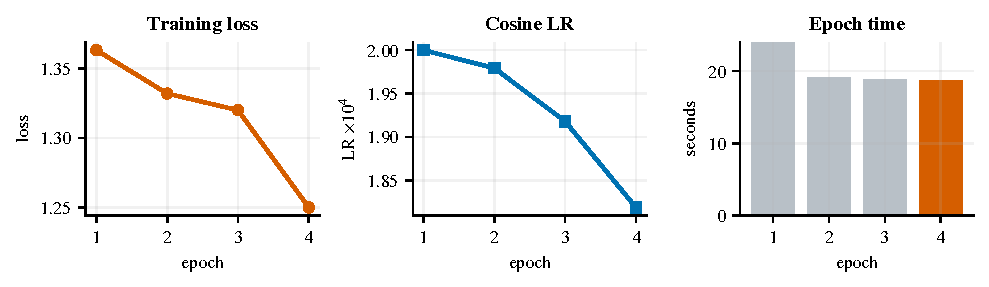
\includegraphics[width=\columnwidth]{fig_training_audit.pdf}
\caption{Training dynamics of the reported D5-512 run: loss, cosine learning rate, and epoch time.
Training stops at epoch 4.}
\label{fig:training}
\end{figure}

\section{Per-epoch Curves and Stopping Regret}
\label{sec:curves}

Every checkpoint of every run was evaluated offline on the full D5 board to validate the online,
metric-free stopping rule (Table~\ref{tab:regret}). The external metric never influences
training. For the main configuration the rule selects the \dinos{} maximum for seeds 42 and 123
and, for seed 7, the epoch that is the maximum of its full 15-epoch curve. For the retrained
ablations, which were run for 15 epochs with stopping disabled, the rule's choice differs from the
oracle: by $6.8\times10^{-5}$ \dinos{} for $\lambda_{LL}=1.0$, but by $0.0039$ for the direct
endpoint, whose peak arrives at epoch 13. The main-paper ablation table therefore reports each
retrained variant at its best-\dinos{} epoch, which is favourable to the variants.

\begin{table}[t]
\centering
\caption{Stopping rule versus \dinos{} oracle on D5-512. $e_{\mathrm{int}}$: epoch chosen by the
internal rule; $e^\ast$: best \dinos{} epoch among evaluated checkpoints.}
\label{tab:regret}
\footnotesize
\setlength{\tabcolsep}{3pt}
\begin{tabular}{@{}lrrrcc@{}}
\toprule
Run & epochs & $e_{\mathrm{int}}$ & $e^\ast$ & \dinos($e^\ast$) & regret \\
\midrule
WEAVE, seed 42 & 4 & 4 & 4 & 0.4917 & 0 \\
WEAVE, seed 7 & 15 & 4$^a$ & 4 & 0.4910 & 0 \\
WEAVE, seed 123 & 3 & 3 & 3 & 0.4862 & 0 \\
$\lambda_{LL}=1.0$ & 15 & 5 & 3 & 0.4910 & $6.8\!\times\!10^{-5}$ \\
direct endpoint & 15 & 5 & 13 & 0.4894 & 0.0039 \\
learned HH head & 15 & 4 & 4 & 0.4930 & 0 \\
\bottomrule
\end{tabular}\\[2pt]
{\scriptsize $^a$relative rule; the superseded absolute rule did not fire for this seed.}
\end{table}

For seed 42, (\dinos, \clips, LPIPS, \dinoc) is (0.4857, 0.7119, 0.2409, 0.8230) after epoch 1,
(0.4887, 0.7158, 0.2625, 0.7978) after epoch 2, (0.4913, 0.7176, 0.2645, 0.7853) after epoch 3, and
(0.4917, 0.7127, 0.2595, 0.8104) after epoch 4. The main table reports a
re-evaluation of the same epoch-4 checkpoint (0.4918/0.7128/0.2595/0.8102); the difference is
below $2\times10^{-4}$ on every metric. After epoch 4, \dinos{} declines while the regression
loss keeps improving, so the transition is not ordinary loss-plateau stopping.

\section{Sensitivity Sweeps}
\label{sec:sweeps}

Table~\ref{tab:sweeps} reports three one-factor sweeps. The AdaIN scale sweep changes only
inference on the reported checkpoint and is fully matched. The $\lambda_{LL}$ and $\alpha$ sweeps
retrain the model at a fixed budget of four to five epochs, whereas the $0.3/0.3$ reference point comes from the
internally stopped main run; the reference row is therefore not a matched member of either sweep
and we do not claim that 0.3 is uniquely optimal. Within $\lambda_{LL}\in[0.1,0.5]$ the \dinos{}
range of the retrained points is 0.4847--0.4857, while \dinoc{} decreases and \clips{} increases
monotonically with $\lambda_{LL}$. Along $\alpha$, \dinoc{} falls and LPIPS also falls, showing that
the two content proxies can disagree, which is why both are reported. AdaIN scale is flat between
1.0 and 1.5 and changes sharply at 2.0, where \dinos{}, \dinoc{}, and LPIPS improve while \clips{}
drops slightly; values above 2.0 were not tested on this checkpoint (on the earlier base model,
scale 2.5 collapses content: \dinoc{} 0.259).

\begin{table}[t]
\centering
\caption{Sensitivity sweeps on D5-512 (\dinos/\dinoc/\clips/LPIPS).}
\label{tab:sweeps}
\footnotesize
\setlength{\tabcolsep}{3.5pt}
\begin{tabular}{@{}lcccc@{}}
\toprule
Setting & \dinos & \dinoc & \clips & LPIPS \\
\midrule
\multicolumn{5}{@{}l}{\emph{Stepwise AdaIN scale $\beta$ (same checkpoint)}} \\
1.0 & 0.4831 & 0.8024 & 0.7165 & 0.2863 \\
1.25 & 0.4838 & 0.8026 & 0.7167 & 0.2865 \\
1.5 & 0.4844 & 0.8031 & 0.7168 & 0.2864 \\
2.0 & 0.4920 & 0.8099 & 0.7126 & 0.2593 \\
\midrule
\multicolumn{5}{@{}l}{\emph{LL loss weight $\lambda_{LL}$ (retrained, fixed budget)}} \\
0.1 & 0.4856 & 0.8206 & 0.7110 & 0.2585 \\
0.15 & 0.4857 & 0.8202 & 0.7111 & 0.2589 \\
0.2 & 0.4856 & 0.8185 & 0.7119 & 0.2598 \\
0.25 & 0.4853 & 0.8178 & 0.7121 & 0.2595 \\
0.35 & 0.4850 & 0.8151 & 0.7135 & 0.2591 \\
0.4 & 0.4847 & 0.8141 & 0.7136 & 0.2575 \\
0.45 & 0.4850 & 0.8122 & 0.7141 & 0.2577 \\
0.5 & 0.4848 & 0.8106 & 0.7143 & 0.2573 \\
\midrule
\multicolumn{5}{@{}l}{\emph{LL blend $\alpha$ in Eq.~(1) (retrained, fixed budget)}} \\
0.1 & 0.4859 & 0.8243 & 0.7096 & 0.2714 \\
0.2 & 0.4864 & 0.8215 & 0.7108 & 0.2651 \\
0.4 & 0.4845 & 0.8090 & 0.7148 & 0.2557 \\
0.5 & 0.4843 & 0.8016 & 0.7152 & 0.2552 \\
\midrule
reference (main run) & 0.4918 & 0.8102 & 0.7128 & 0.2595 \\
\bottomrule
\end{tabular}
\end{table}

\section{Reference-pool Stability}
\label{sec:refpool}

Without regenerating images, we draw for each target style one size-$m$ subset of its 30 held-out
references without replacement, reuse it for all 150 requests to that style, and recompute
\dinos{} for WEAVE and IDT; this is repeated 1{,}000 times (Table~\ref{tab:refpool}). Absolute
\dinos{} grows with $m$ because it is a maximum over the pool, but the board-mean margin over IDT is
positive in every repetition. Roughly 69\% of individual requests have a positive margin, so the
evidence supports a board-level conclusion rather than a per-image guarantee.

\begin{table}[t]
\centering
\caption{\dinos{} under reference-pool resampling (1{,}000 draws, D5-512).}
\label{tab:refpool}
\footnotesize
\setlength{\tabcolsep}{3pt}
\begin{tabular}{@{}rcccc@{}}
\toprule
$m$ & WEAVE & IDT & margin (95\% interval) & positive \\
\midrule
8 & 0.345 & 0.315 & 0.0298 [0.0204, 0.0394] & 100\% / 68.9\% \\
16 & 0.378 & 0.346 & 0.0319 [0.0225, 0.0380] & 100\% / 69.2\% \\
30 & 0.403 & 0.370 & 0.0334 (full pool) & -- \\
\bottomrule
\end{tabular}\\[2pt]
{\scriptsize ``positive'': fraction of draws with positive board margin / of individual requests.}
\end{table}

\section{ArtFID Audit}
\label{sec:artfid}

ArtFID is computed per target style as $(1+\mathrm{FID})(1+\mathrm{LPIPS})$ and averaged over
targets on a single 750-request source manifest (Table~\ref{tab:artfid}). Only methods whose
outputs match that manifest are compared; Z-STAR and StyleAligned outputs were produced from a
different source list and are excluded, and Seedream (API) covers 720 requests and is shown for
reference. IDT obtains the best ArtFID and also the best raw FID, so ArtFID alone cannot
distinguish successful transfer from no transfer; this motivates the IDT reference. WEAVE and
SaMam are close on ArtFID, but WEAVE clears IDT on \clips{} while SaMam does not (main Table I; its CLIP-S is below IDT on D5 and R5).

\begin{table}[t]
\centering
\caption{Target-pooled ArtFID on D5-512 (lower is better).}
\label{tab:artfid}
\footnotesize
\begin{tabular}{@{}lrrr@{}}
\toprule
Method & FID & LPIPS & ArtFID \\
\midrule
IDT & 215.5 & 0.000 & 216.5 \\
WEAVE & 230.5 & 0.283 & 295.3 \\
SaMam & 231.9 & 0.283 & 297.3 \\
Seedream 4.5 (720 req.) & 217.4 & 0.422 & 311.0 \\
TGT (30 random draws) & 305.3 & 0.787 & 545.7 $\pm$ 56.1 \\
\bottomrule
\end{tabular}
\end{table}

\section{Structure Preservation}
\label{sec:structure}

As a geometry check independent of DINO and LPIPS, we compare MiDaS (DPT) depth maps and Canny edge maps
of source and output on all 750 D5 requests. WEAVE has a lower depth MSE than SaMam (0.0321 vs.\
0.0406; median 0.0182 vs.\ 0.0216), while SaMam has a higher edge IoU (0.159 vs.\ 0.140), consistent
with WEAVE re-texturing edges while keeping scene depth. StyleAligned outputs were available for
only 15 matched requests (depth MSE 0.129, edge IoU 0.004) and are indicative only.

\section{High-frequency Route Probes}
\label{sec:probes}

Before the final architecture was fixed, we diagnosed why the base model moved style weakly. The
structure-aligned target already requests target high frequencies, but in the base model the
target latent shapes the supervision without entering the velocity predictor as an image-specific
condition. We therefore fine-tuned alternative target-HF routes from one base checkpoint (AdaIN
scale 1.5, D5 board; diagnostic only, not mixed into the main table), see Table~\ref{tab:routes}
and Fig.~\ref{fig:routes}. Raw spatial target maps raise style but leak target layout
(\dinoc{} 0.404, LPIPS 0.538). Pooled subband codes keep content while raising style; zeroing them
at inference lowers both \dinos{} and \dinoc{}, so the route is causal. Scaling the route (1.25$\times$,
1.5$\times$) trades content for off-diagonal style without improving the balanced point, and a
direction auxiliary improves a decomposition probe but hurts image metrics. The final model uses
orientation-specific pooled codes for LH and HL only.

\begin{table}[t]
\centering
\caption{Target-HF route probes (fine-tunes of one base checkpoint, D5-512).}
\label{tab:routes}
\footnotesize
\setlength{\tabcolsep}{3pt}
\begin{tabular}{@{}lcccc@{}}
\toprule
Route & \dinos & \dinoc & LPIPS & \clips \\
\midrule
HF delta, 15 epochs & 0.4825 & 0.7913 & 0.2991 & 0.7180 \\
raw spatial target HF & 0.4901 & 0.4043 & 0.5382 & 0.7483 \\
pooled subband codes & 0.4886 & 0.7981 & 0.2966 & 0.7209 \\
\;codes zeroed at inference & 0.4858 & 0.7888 & 0.3010 & 0.7205 \\
\;codes $\times$1.5 & 0.4875 & 0.7798 & 0.3054 & 0.7211 \\
subband + texture stats & 0.4884 & 0.7988 & 0.2960 & 0.7194 \\
without style memory & 0.4849 & 0.7948 & 0.2943 & 0.7167 \\
direction auxiliary & 0.4862 & 0.7939 & 0.2974 & 0.7189 \\
\bottomrule
\end{tabular}
\end{table}

\begin{figure}[t]
\centering
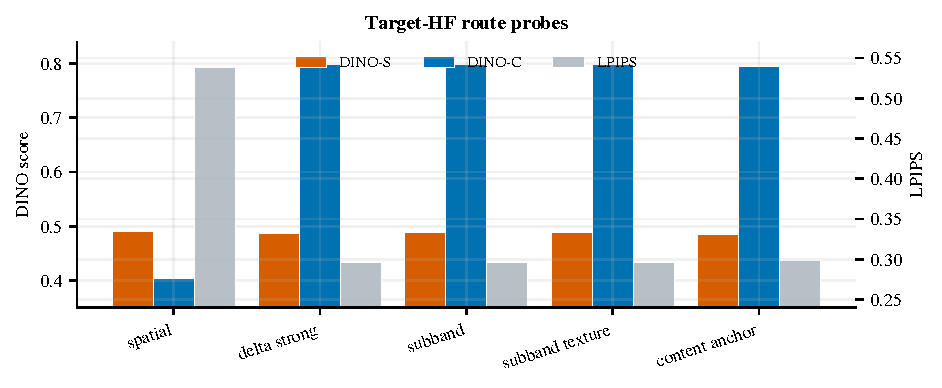
\includegraphics[width=\columnwidth]{fig_probe_mechanisms.pdf}
\caption{Target-HF route probes. Spatial injection raises style but collapses content; pooled
subband routes keep content at nearly the same style level.}
\label{fig:routes}
\end{figure}

\section{Additional Comparisons}
\label{sec:more}

Fig.~\ref{fig:tradeoff} places all D5 methods on the style/content plane and Fig.~\ref{fig:cost}
shows training and inference cost of the learned methods. Fig.~\ref{fig:radar} summarizes all three
boards; each metric family is min--max normalized once across methods and boards and speed uses
$\log_{10}(1+t)$, so the radar is a visual summary of Table I and not a composite score.

\noindent\textbf{Unseen families.} The five held-out WikiArt families are disjoint from D5; all
methods use their D5 checkpoints and the same 750-request layout (Table III of the main paper).

\noindent\textbf{Frozen SD1.5 plug-in.} The control is an SD1.5 image-to-image pipeline with an
empty prompt, strength 0.5, and 20 DDIM steps. The plug-in applies a one-level Haar transform to
the output latent, aligns the channel moments of LH, HL, and HH to the target-style latent at scale
0.8, leaves LL unchanged, and inverts the transform. On all 750 requests (including same-style
rows), \dinos{} changes from 0.4525 to 0.4613 and \clips{} from 0.7476 to 0.7594, while LPIPS stays
at 0.3586/0.3588 and \dinoc{} moves from 0.6583 to 0.6539. The operation costs 4.9\,ms per image
(720 timed requests). The experiment isolates the portability of the frequency-domain operator; it
does not equate the compact model with SD1.5.

\begin{figure}[t]
\centering
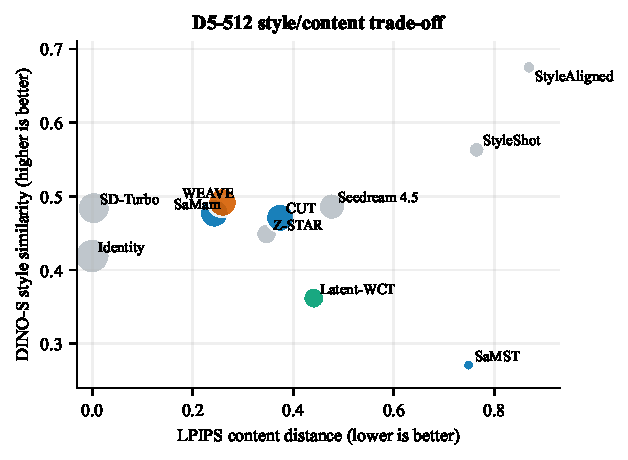
\includegraphics[width=0.9\columnwidth]{fig_d5_tradeoff.pdf}
\caption{D5-512 style/content plane. WEAVE is not the maximum-style point but lies in the
low-LPIPS region among methods that clear the IDT style reference.}
\label{fig:tradeoff}
\end{figure}

\begin{figure}[t]
\centering
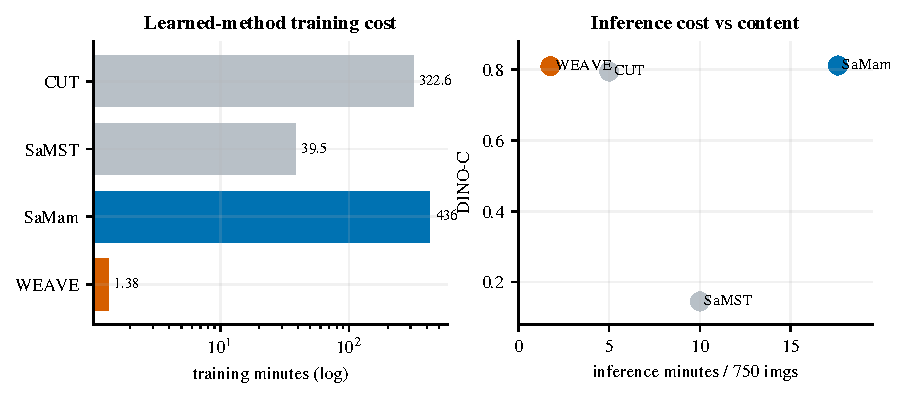
\includegraphics[width=\columnwidth]{fig_cost_quality.pdf}
\caption{Training minutes (left, log scale) and inference minutes versus \dinoc{} (right) for the
learned methods.}
\label{fig:cost}
\end{figure}

\begin{figure}[t]
\centering
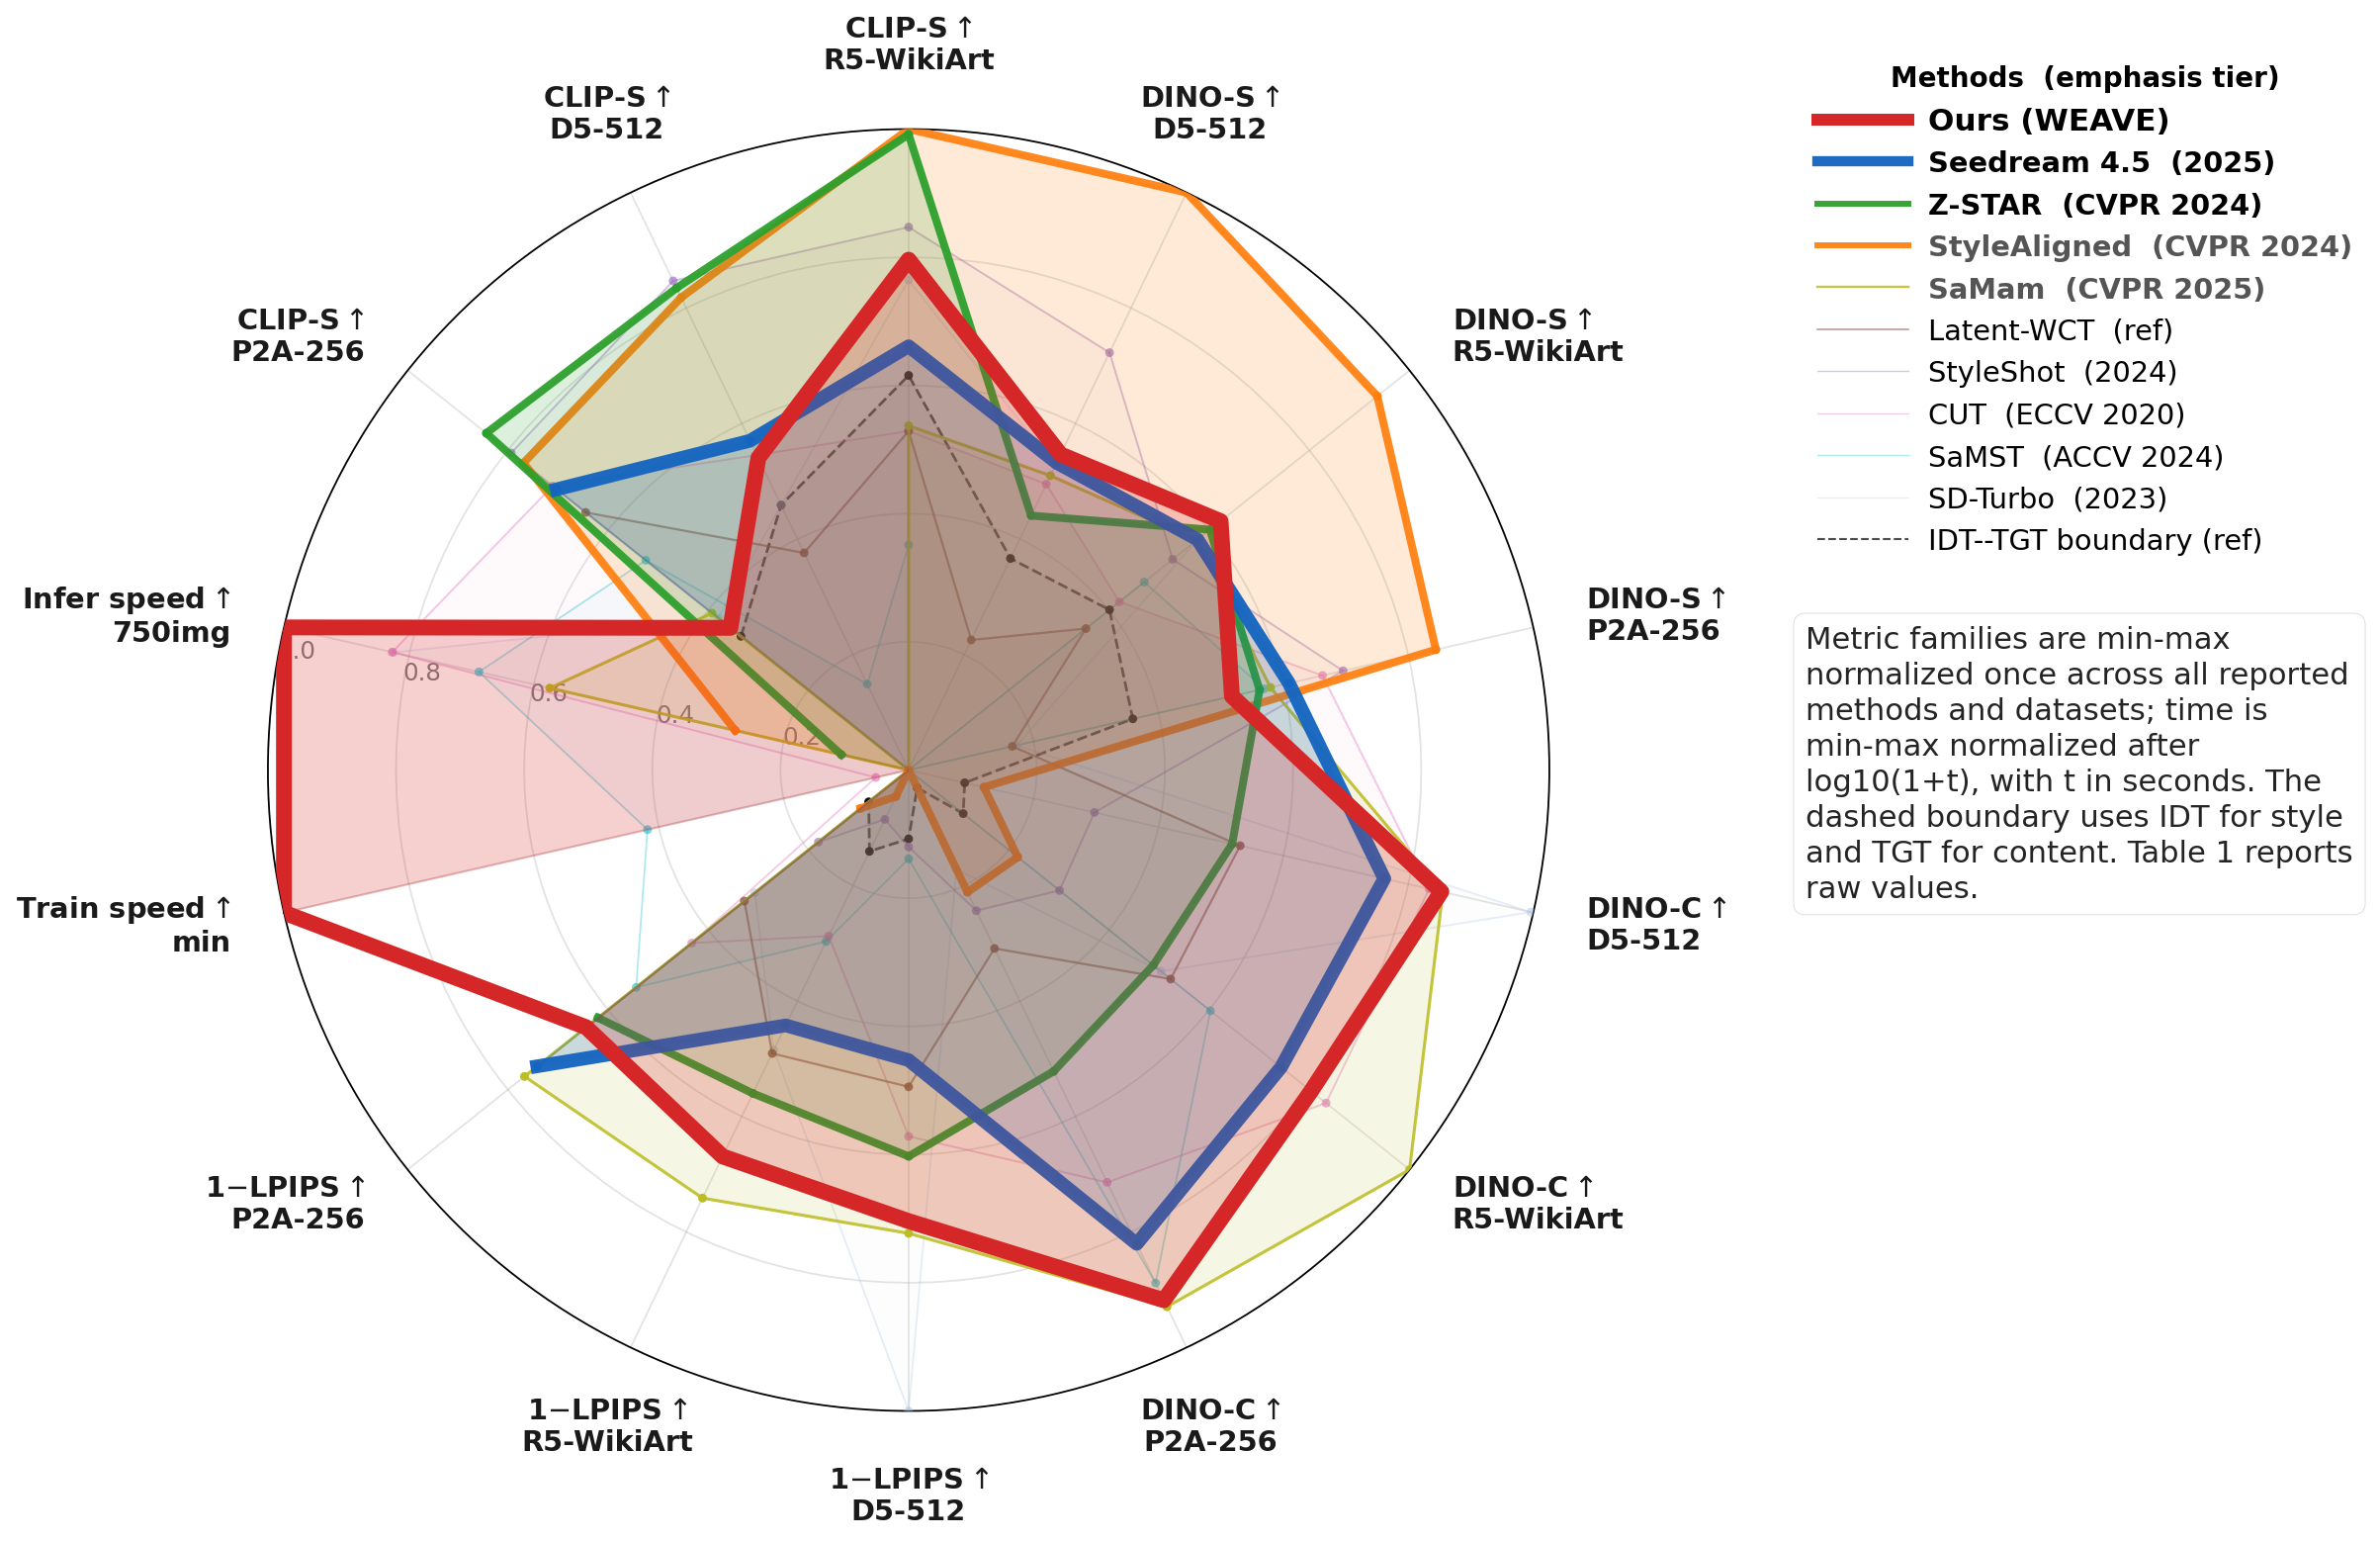
\includegraphics[width=\columnwidth]{radar_metric_blocks_A_clip_dinos_robustbreak.png}
\caption{Style, content, and cost across the three boards. The dashed boundary uses IDT on style
axes and TGT on content axes.}
\label{fig:radar}
\end{figure}

\section{Ethics and Reproducibility}
\label{sec:ethics}

Style transfer can be misused to produce deceptive images or misattribute authorship. WEAVE
operates at the level of style families (e.g., Impressionism) and does not model or label
individual artists, although inference uses target-style reference images. All data are public
WikiArt artworks without personal data, and the VAE is the public SD1.5 EMA VAE. Code, the
selected checkpoint, and the 750-request manifests will be released upon publication. Reported
training time starts after one-off latent caching; inference time includes VAE decoding.

\end{document}
